\documentclass[aspectratio=169,11pt]{beamer}
% Shared Beamer setup for Ms Economía PEG, Problem Set 1, Team 3.
\usepackage[T1]{fontenc}
\usepackage[utf8]{inputenc}
\usepackage[spanish,es-noshorthands]{babel}
\usepackage{booktabs}
\usepackage{graphicx}
\usepackage{amsmath,amssymb}
\usepackage{tabularx}
\usepackage{xcolor}
\usepackage{tikz}
\usepackage{hyperref}

\graphicspath{{../02_outputs/figures/}{img/}{./}}
\newcommand{\nsample}{14,761}
\newcommand{\ntrain}{10,260}
\newcommand{\nvalid}{4,501}
\newcommand{\sharefemale}{47.3}
\newcommand{\medianincome}{992,745}
\newcommand{\meanincome}{1,617,237}
\newcommand{\medianhours}{48}
\newcommand{\meanage}{38.9}
\newcommand{\peakuncond}{40.6}
\newcommand{\peakuncondlo}{40.1}
\newcommand{\peakuncondhi}{41.2}
\newcommand{\peakcond}{43.6}
\newcommand{\peakcondlo}{42.8}
\newcommand{\peakcondhi}{44.5}
\newcommand{\rtwoageu}{0.050}
\newcommand{\rtwoagec}{0.226}
\newcommand{\gapuncond}{-21.2}
\newcommand{\gaphc}{-27.2}
\newcommand{\gappref}{-19.6}
\newcommand{\gapjob}{-18.9}
\newcommand{\gapcoef}{-0.218}
\newcommand{\gapse}{0.012}
\newcommand{\gapseboot}{0.012}
\newcommand{\fwlcoef}{-0.218}
\newcommand{\peakmen}{50.5}
\newcommand{\peakmenlo}{49.1}
\newcommand{\peakmenhi}{52.3}
\newcommand{\peakwomen}{45.6}
\newcommand{\peakwomenlo}{44.4}
\newcommand{\peakwomenhi}{47.0}
\newcommand{\bestmodel}{P6: Flexible age, education, and hours}
\newcommand{\bestshort}{P6: polinomio flexible}
\newcommand{\gapuncondabs}{21.2}
\newcommand{\gaphcabs}{27.2}
\newcommand{\gapprefabs}{19.6}
\newcommand{\bestvalid}{0.6160}
\newcommand{\bestloocv}{0.5825}
\newcommand{\besttrain}{0.5797}
\newcommand{\topvar}{Socioeconomic stratum}
\newcommand{\topdelta}{0.1185}


\definecolor{navy}{HTML}{1B365D}
\definecolor{accent}{HTML}{B85C38}
\definecolor{slate}{HTML}{5B6B73}
\definecolor{gold}{HTML}{C4A35A}
\definecolor{ice}{HTML}{F4F6F8}

\setbeamercolor{structure}{fg=navy}
\setbeamercolor{frametitle}{fg=navy,bg=white}
\setbeamercolor{title}{fg=navy}
\setbeamercolor{subtitle}{fg=slate}
\setbeamercolor{author}{fg=slate}
\setbeamercolor{institute}{fg=slate}
\setbeamercolor{date}{fg=slate}
\setbeamercolor{item}{fg=accent}
\setbeamercolor{footline}{fg=slate}
\setbeamercolor{normal text}{fg=navy}

\setbeamertemplate{navigation symbols}{}
\setbeamertemplate{itemize items}[circle]
\setbeamerfont{frametitle}{series=\bfseries,size=\large}
\setbeamerfont{title}{series=\bfseries,size=\LARGE}

% Escudo Uniandes: portada y esquina superior derecha de cada diapositiva.
\newcommand{\uniandeslogo}[1][0.92cm]{
\includegraphics[height=#1]{logo_uniandes.png}}

\setbeamertemplate{frametitle}{%
  \nointerlineskip
  \vspace{0.18cm}%
  \leavevmode
  \hbox to \textwidth{%
    \begin{minipage}[c]{0.88\textwidth}
      \raggedright
      \usebeamerfont{frametitle}\usebeamercolor[fg]{frametitle}\insertframetitle
    \end{minipage}%
    \hfil
    \raisebox{-0.12cm}{\uniandeslogo[0.72cm]}%
  }%
  \vspace{0.12cm}%
}

\setbeamertemplate{title page}{%
  \vbox{}
  \vspace{0.15cm}
  \begin{flushright}
    \uniandeslogo[1.15cm]
    \hspace{0.08cm}
  \end{flushright}
  \vspace{0.55cm}
  \begin{center}
    {\usebeamerfont{title}\usebeamercolor[fg]{title}\inserttitle\par}
    \vspace{0.45em}
    {\usebeamerfont{subtitle}\usebeamercolor[fg]{subtitle}\insertsubtitle\par}
    \vspace{1.15em}
    {\usebeamerfont{author}\insertauthor\par}
    \vspace{0.55em}
    {\usebeamerfont{institute}\insertinstitute\par}
    \vspace{0.85em}
    {\usebeamerfont{date}\insertdate\par}
  \end{center}
}

\setbeamertemplate{footline}{
  \leavevmode%
  \hbox{%
    \begin{beamercolorbox}[wd=.55\paperwidth,ht=2.4ex,dp=1.2ex,leftskip=1em]{footline}
      \tiny Grupo 3 $\cdot$ Ms Economía PEG $\cdot$ Universidad de los Andes
    \end{beamercolorbox}%
    \begin{beamercolorbox}[wd=.45\paperwidth,ht=2.4ex,dp=1.2ex,rightskip=1em,right]{footline}
      \tiny \insertframenumber/\inserttotalframenumber
    \end{beamercolorbox}}%
  \vskip0pt%
}

\newcommand{\statblock}[3]{%
  \begin{tikzpicture}
    \node[fill=ice, inner sep=10pt, text width=0.42\textwidth, align=center] {
      {\fontsize{20}{24}\selectfont\bfseries\color{navy} #1}\\[4pt]
      {\small\color{slate} #2}\\[2pt]
      {\scriptsize\color{accent} #3}
    };
  \end{tikzpicture}%
}

\newcommand{\source}[1]{\vfill{\scriptsize\color{slate} #1}}


\title{Perfil edad--ingreso laboral}
\subtitle{Taller 1 $\cdot$ Secci\'on 1}
\author{Juli\'an Herrera \and Andr\'es Silva \and Valentina Vera}
\institute{Ms Econom\'ia PEG $\cdot$ Big Data and Machine Learning para Econom\'ia Aplicada\\ Universidad de los Andes}
\date{2026-20 $\cdot$ Grupo 3}

\begin{document}

\begin{frame}[plain]
  \titlepage
\end{frame}

\begin{frame}{Visi\'on general}
  \textbf{Pregunta.} ¿Puede un perfil edad--ingreso servirle a la autoridad tributaria como referencia de lo que es \emph{esperable} declarar a cada edad ---y d\'onde esa referencia deja de servir?

  \vspace{0.65em}
  \textbf{Relevancia.} El subreporte de ingreso laboral es un canal cl\'asico de la brecha tributaria. Sin una referencia de ciclo de vida, el auditor compara a un trabajador de 30 a\~nos con uno de 50 como si el mercado pagara lo mismo. No lo hace: el capital humano predice que el ingreso sube, llega a un pico y luego se aplana o cae.

  \vspace{0.65em}
  \textbf{Desaf\'io en la pr\'actica.} Un perfil crudo mezcla productividad, horas y tipo de empleo. Un filtro ingenuo marca como sospechoso a quien trabaja medio tiempo o por cuenta propia. La edad organiza el ingreso, pero no lo determina: el residual de cualquier perfil es espacio de auditor\'ia, no una prueba de evasi\'on.

  \vspace{0.5em}
  Esta secci\'on estima esa forma ---incondicional y condicional en horas y tipo de ocupaci\'on--- y discute qu\'e se le puede pedir a ese perfil, y qu\'e no.
  \source{Ocupados de 18 a\~nos o m\'as, Bogot\'a, GEIH 2018.}
\end{frame}

\begin{frame}{La evidencia descriptiva ya muestra la U invertida}
  \begin{center}
    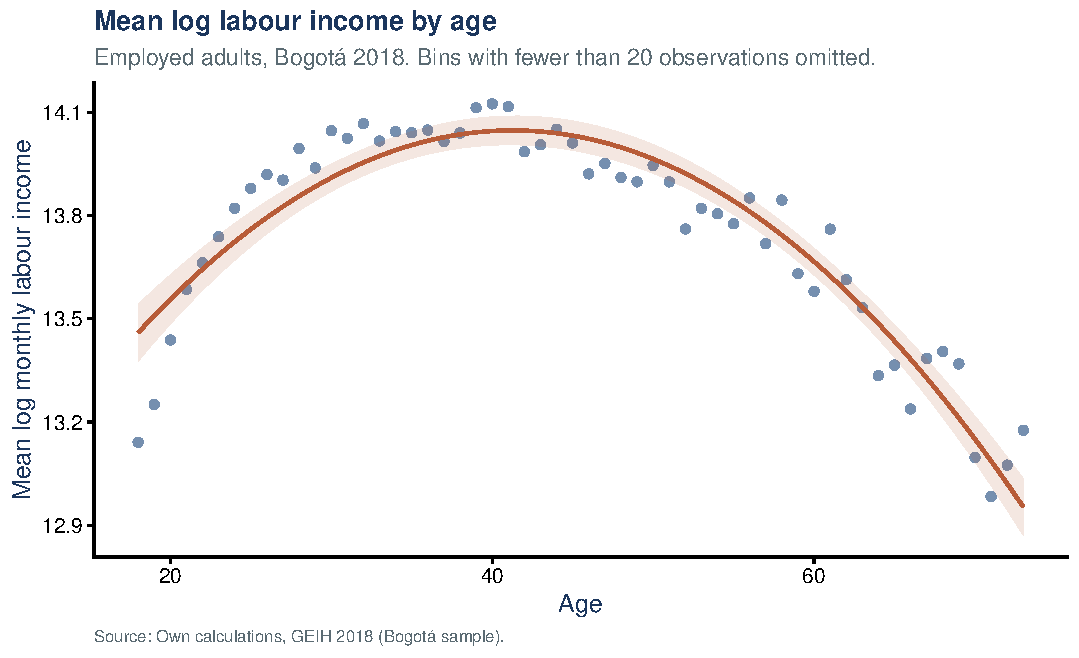
\includegraphics[width=0.92\textwidth]{fig_age_binned_means.pdf}
  \end{center}
\end{frame}

\begin{frame}{Especificaciones}
  \begin{align*}
    \log(w_i) &= \beta_1 + \beta_2 \mathrm{Edad}_i + \beta_3 \mathrm{Edad}_i^2 + u_i \\[4pt]
    \log(w_i) &= \beta_1 + \beta_2 \mathrm{Edad}_i + \beta_3 \mathrm{Edad}_i^2 + \gamma \mathrm{Horas}_i + \delta' \mathrm{Relab}_i + u_i
  \end{align*}
  \vspace{0.3em}
  \begin{itemize}
    \item Pico impl\'icito: $\mathrm{edad}^*=-\beta_2/(2\beta_3)$, si $\beta_3<0$.
    \item Intervalo de confianza por \textbf{bootstrap} de la muestra ($R=5000$), no por el m\'etodo delta: $\mathrm{edad}^*$ es no lineal en los coeficientes.
    \item Horas y tipo de ocupaci\'on (\texttt{relab}) son los \emph{\'unicos} controles. Capturan el margen intensivo y la posici\'on ocupacional.
  \end{itemize}
\end{frame}

\begin{frame}{Estimaci\'on: pico, intervalo y ajuste}
  \begin{center}
    \footnotesize
    \begin{tabular}{lccccc}
\toprule
Specification & Peak age & 95\% bootstrap CI & R$^2$ & Adj. R$^2$ & N \\
\midrule
Unconditional & 40.6 & [40.1, 41.2] & 0.050 & 0.050 & 14,761 \\
Conditional & 43.6 & [42.8, 44.5] & 0.226 & 0.226 & 14,761 \\
\bottomrule
\end{tabular}

  \end{center}
  \vspace{0.6em}
  \begin{itemize}
    \item Ambos picos caen \textbf{dentro} del rango de edad observado. El perfil no es solo creciente.
    \item Condicionar en horas y tipo de ocupaci\'on cambia el pico: parte del perfil crudo es composici\'on (qui\'en trabaja m\'as horas a cada edad).
    \item El $R^2$ sigue siendo bajo. La edad organiza el ingreso; no lo determina.
  \end{itemize}
  \source{Errores est\'andar anal\'iticos en el repositorio. IC del pico: bootstrap i.i.d., 5.000 r\'eplicas.}
\end{frame}

\begin{frame}{Perfiles predichos}
  \begin{center}
    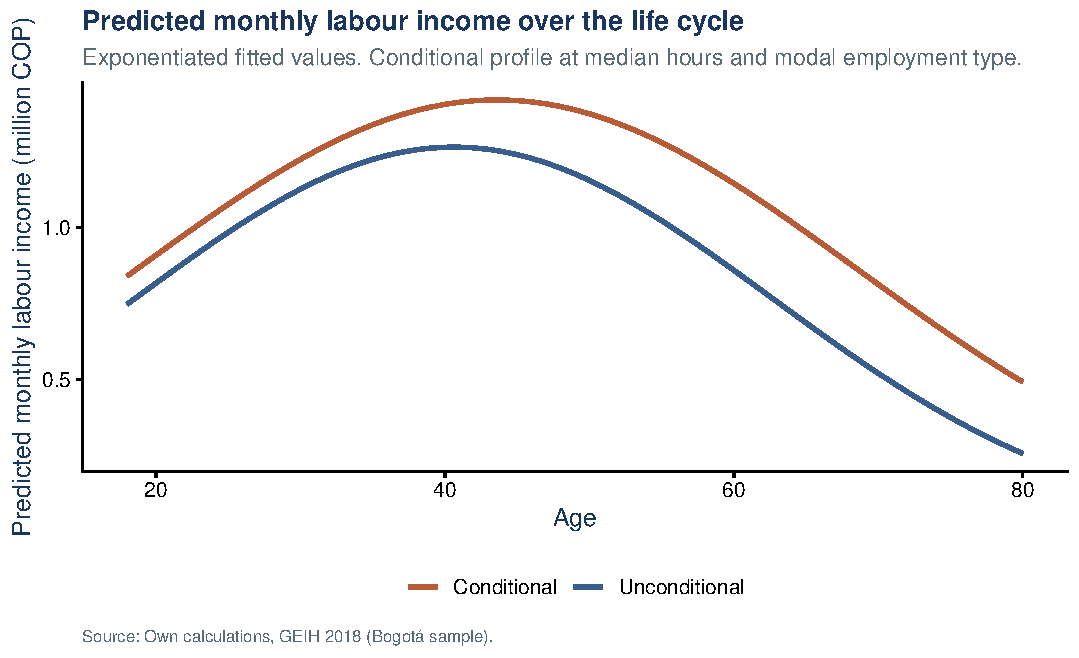
\includegraphics[width=0.92\textwidth]{fig_age_profiles_cop.pdf}
  \end{center}
\end{frame}

\begin{frame}{Lectura para la autoridad tributaria}
  \begin{itemize}
    \item Un asalariado de 30 a\~nos y uno de 50 \textbf{no} deber\'ian compararse con la misma referencia. El modelo da la referencia por edad.
    \item Condicionar en horas evita marcar como subdeclarante a quien trabaja medio tiempo.
    \item Condicionar en tipo de ocupaci\'on evita confundir cuenta propia con asalariado privado.
    \item Lo que el modelo \textbf{no} ve ---educaci\'on, formalidad, estrato--- aparece en el residual. Ah\'i es donde la Secci\'on 3 mide el error de predicci\'on.
  \end{itemize}
  \vspace{0.8em}
  \begin{block}{En s\'intesis}
    El pico a los \peakuncond\ a\~nos (IC [\peakuncondlo, \peakuncondhi]) es el hecho descriptivo. El perfil condicional lo desplaza a \peakcond, pero conserva la U invertida. La autoridad puede usar esa forma; no puede usarla sola.
  \end{block}
\end{frame}

\end{document}
